% Illustrations of the six beams for the README (one page per beam).
% Build: latexmk -pdf beams.tex && pdftoppm -r 150 -png beams.pdf tmp, then rename tmp-1..6.png to beam_A..F.png
% Colours follow the figures of theory/nonparax.tex.
\documentclass[tikz,multi=tikzpicture,border=4pt]{standalone}
\usepackage[T1]{fontenc}
\usetikzlibrary{arrows.meta,calc,decorations.markings}
\definecolor{capl}{HTML}{0072B2}    % aplanatic objective
\definecolor{cthin}{HTML}{D55E00}   % thin lens
\definecolor{cspec}{HTML}{009E73}   % Gaussian spectrum

\tikzset{
  every picture/.style={>=Latex, font=\small},
  ray/.style={thick, postaction={decorate},
    decoration={markings, mark=at position 0.5 with {\arrow{>}}}},
  pw/.style={cspec, postaction={decorate},
    decoration={markings, mark=at position 0.6 with {\arrow{>}}}},
}
\def\f{1.9}       % focal length = radius of the reference sphere
\def\xp{-3.0}     % pupil plane
\def\wap{1.0}     % 1/e radius of the pupil Gaussian
\def\rtwo{1.55}   % stop radius
\def\kwz{3}       % k w0 for the plane-wave weights

% ---------------------------------------------------------------- shared pieces
\newcommand{\spectrum}{%
  \draw[->,thick] (-2.8,0) -- (1.2,0);
  \draw[dotted] (100:2.3) arc (100:260:2.3);
  \foreach \t in {0,20,40,60,75,-20,-40,-60,-75}{
    \pgfmathsetmacro{\amp}{exp(-(\kwz*sin(\t)/2)^2)}
    \pgfmathsetmacro{\lw}{0.25+1.5*\amp}
    \draw[pw,line width=\lw pt] ({180-\t}:2.3) -- ({180-\t}:0.45);
  }
  \draw[->,thick] (180:2.55) arc (180:140:2.55);
  \node at (160:2.82) {$\theta$};
  \draw[dashed] (0,-2) -- (0,2);
  \fill[cspec!25] plot[domain=-1.9:1.9,samples=60] ({0.7*exp(-(\x/0.75)^2)},\x) -- (0,-1.9) -- cycle;
  \draw[thick,cspec!70!black] plot[domain=-1.9:1.9,samples=60] ({0.7*exp(-(\x/0.75)^2)},\x);
  \draw[<->] (1.0,0) -- (1.0,0.75) node[pos=0.5,right] {$w_0$};
  \fill (0,0) circle (1.1pt);
}
\newcommand{\pupil}{% Gaussian pupil field, no stop
  \draw[->,thick] (-3.8,0) -- (0.9,0);
  \fill[gray!25] plot[domain=-1.9:1.9,samples=60] ({\xp-0.6*exp(-(\x/\wap)^2)},\x) -- (\xp,-1.9) -- cycle;
  \draw[thick] plot[domain=-1.9:1.9,samples=60] ({\xp-0.6*exp(-(\x/\wap)^2)},\x);
  \draw[dashed] (\xp,-2) -- (\xp,2);
  \draw[<->] (\xp-0.72,0) -- (\xp-0.72,\wap) node[pos=0.5,left] {$w_\mathrm{ap}$};
  \fill (0,0) circle (1.1pt);
}
\newcommand{\bbox}{\path[use as bounding box] (-4.6,-2.4) rectangle (2.2,2.75);}

\begin{document}

% ---------------------------------------------------------------- A: Gaussian spectrum
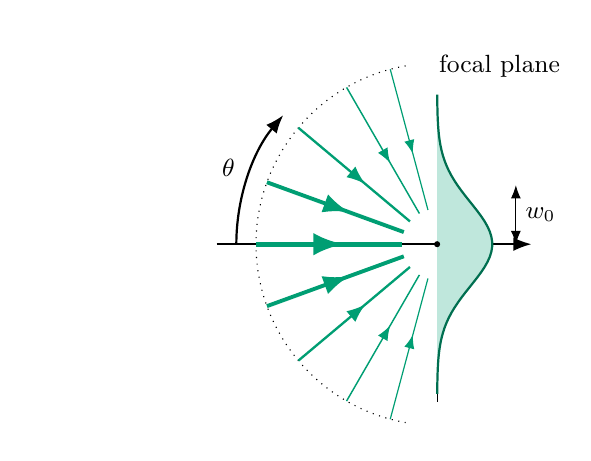
\begin{tikzpicture}
  \bbox
  \begin{scope}[shift={(0.6,0)}]
    \spectrum
    \node[above right] at (-0.1,2) {focal plane};
  \end{scope}
\end{tikzpicture}

% ---------------------------------------------------------------- B: aplanatic objective
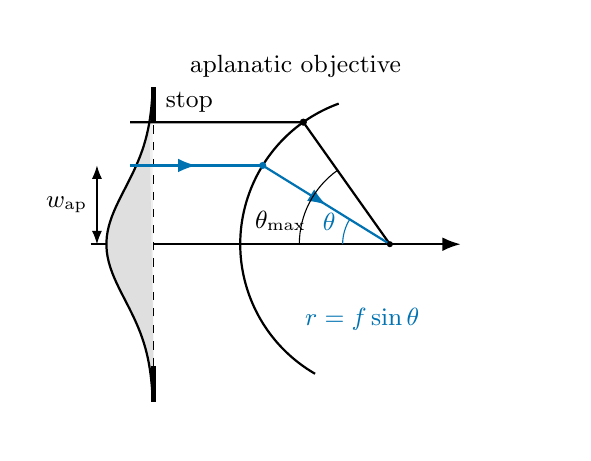
\begin{tikzpicture}
  \bbox
  \pgfmathsetmacro{\thz}{asin(\wap/\f)}
  \pgfmathsetmacro{\thm}{asin(\rtwo/\f)}
  \pgfmathsetmacro{\xz}{-\f*cos(\thz)}
  \pgfmathsetmacro{\xm}{-\f*cos(\thm)}
  \draw[->,thick] (-3.8,0) -- (0.9,0);
  \fill[gray!12] plot[domain=-1.9:1.9,samples=60] ({\xp-0.6*exp(-(\x/\wap)^2)},\x) -- (\xp,-1.9) -- cycle;
  \fill[gray!25] plot[domain=-\rtwo:\rtwo,samples=60] ({\xp-0.6*exp(-(\x/\wap)^2)},\x) -- (\xp,-\rtwo) -- cycle;
  \draw[thick] plot[domain=-1.9:1.9,samples=60] ({\xp-0.6*exp(-(\x/\wap)^2)},\x);
  \draw[dashed] (\xp,-\rtwo) -- (\xp,\rtwo);
  \draw[line width=2pt] (\xp,\rtwo) -- (\xp,2);
  \draw[line width=2pt] (\xp,-\rtwo) -- (\xp,-2);
  \node[right] at (\xp+0.03,1.8) {stop};
  \draw[<->] (\xp-0.72,0) -- (\xp-0.72,\wap) node[pos=0.5,left] {$w_\mathrm{ap}$};
  \draw[thick] (110:\f) arc (110:240:\f);
  \node[above] at (-1.2,2) {aplanatic objective};
  \draw[thick] (\xp-0.3,\rtwo) -- (\xm,\rtwo) -- (0,0);
  \draw[ray,capl] (\xp-0.3,\wap) -- (\xz,\wap);
  \draw[ray,capl] (\xz,\wap) -- (0,0);
  \fill[capl] (\xz,\wap) circle (1.3pt);
  \fill (\xm,\rtwo) circle (1.3pt);
  \node[capl] at (-0.35,-0.95) {$r=f\sin\theta$};
  \draw[capl] (180:0.6) arc (180:{180-\thz}:0.6);
  \node[capl] at (160:0.82) {$\theta$};
  \draw (180:1.15) arc (180:{180-\thm}:1.15);
  \node at (168:1.42) {$\theta_{\max}$};
  \fill (0,0) circle (1.1pt);
\end{tikzpicture}

% ---------------------------------------------------------------- C: thin lens
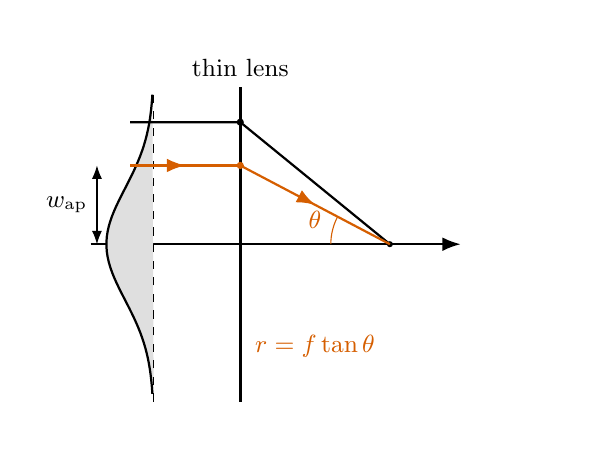
\begin{tikzpicture}
  \bbox
  \pgfmathsetmacro{\tha}{atan(\wap/\f)}
  \pupil
  \draw[line width=1.2pt] (-\f,-2) -- (-\f,2);
  \node[above] at (-\f,2) {thin lens};
  \draw[thick] (\xp-0.3,\rtwo) -- (-\f,\rtwo) -- (0,0);
  \draw[ray,cthin] (\xp-0.3,\wap) -- (-\f,\wap);
  \draw[ray,cthin] (-\f,\wap) -- (0,0);
  \fill[cthin] (-\f,\wap) circle (1.3pt);
  \fill (-\f,\rtwo) circle (1.3pt);
  \node[cthin] at (-0.95,-1.3) {$r=f\tan\theta$};
  \draw[cthin] (180:0.75) arc (180:{180-\tha}:0.75);
  \node[cthin] at (162:1.0) {$\theta$};
\end{tikzpicture}

% ---------------------------------------------------------------- D: COMSOL
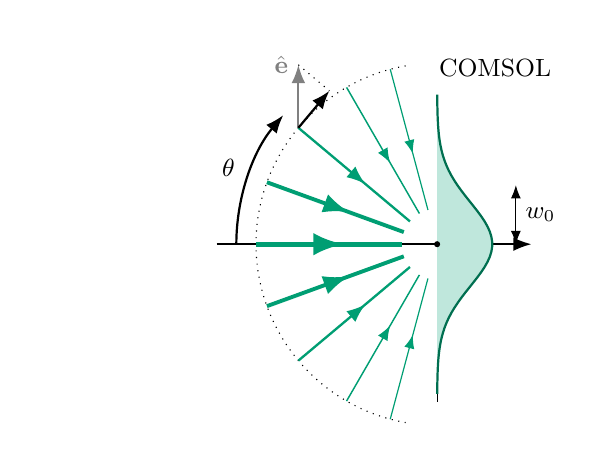
\begin{tikzpicture}
  \bbox
  \begin{scope}[shift={(0.6,0)}]
    \spectrum
    % projection of the input polarization normal to one plane wave (theta = 40 deg)
    \coordinate (P) at (140:2.3);
    \draw[->,thick,gray] (P) -- ++(0,0.8) node[left] {$\hat{\mathbf e}$};
    \draw[->,thick] (P) -- ++({0.8*sin(40)*cos(40)},{0.8*cos(40)*cos(40)});
    \draw[dotted] ($(P)+(0,0.8)$) -- ($(P)+({0.8*sin(40)*cos(40)},{0.8*cos(40)*cos(40)})$);
    \node[above right] at (-0.1,2) {COMSOL};
  \end{scope}
\end{tikzpicture}

% ---------------------------------------------------------------- E: OTT sintheta
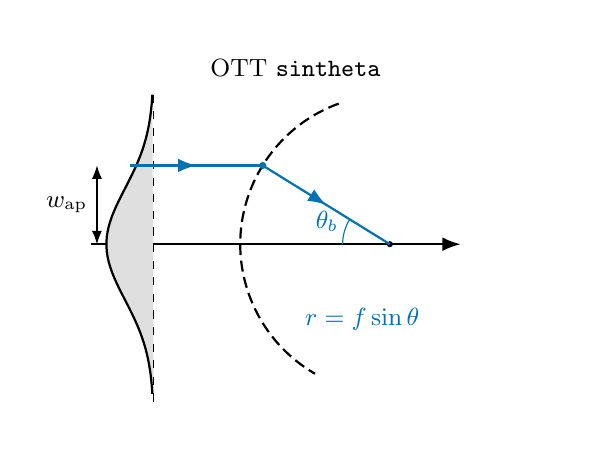
\begin{tikzpicture}
  \bbox
  \pgfmathsetmacro{\thz}{asin(\wap/\f)}
  \pgfmathsetmacro{\xz}{-\f*cos(\thz)}
  \pupil
  \draw[thick,dash pattern=on 4pt off 2pt] (110:\f) arc (110:240:\f);
  \node[above] at (-1.2,2) {OTT \texttt{sintheta}};
  \draw[ray,capl] (\xp-0.3,\wap) -- (\xz,\wap);
  \draw[ray,capl] (\xz,\wap) -- (0,0);
  \fill[capl] (\xz,\wap) circle (1.3pt);
  \node[capl] at (-0.35,-0.95) {$r=f\sin\theta$};
  \draw[capl] (180:0.6) arc (180:{180-\thz}:0.6);
  \node[capl] at (160:0.85) {$\theta_b$};
\end{tikzpicture}

% ---------------------------------------------------------------- F: OTT tantheta
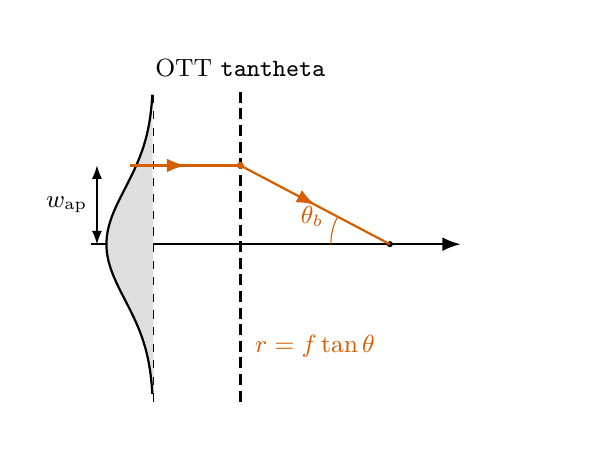
\begin{tikzpicture}
  \bbox
  \pgfmathsetmacro{\tha}{atan(\wap/\f)}
  \pupil
  \draw[line width=1.2pt,dash pattern=on 4pt off 2pt] (-\f,-2) -- (-\f,2);
  \node[above] at (-\f,2) {OTT \texttt{tantheta}};
  \draw[ray,cthin] (\xp-0.3,\wap) -- (-\f,\wap);
  \draw[ray,cthin] (-\f,\wap) -- (0,0);
  \fill[cthin] (-\f,\wap) circle (1.3pt);
  \node[cthin] at (-0.95,-1.3) {$r=f\tan\theta$};
  \draw[cthin] (180:0.75) arc (180:{180-\tha}:0.75);
  \node[cthin] at (160:1.05) {$\theta_b$};
\end{tikzpicture}

\end{document}
